\section{Specifica della componente presenter}
Questa componente consente la gestione della logica principale dell'applicazione \progetto{} e viene suddivisa in due parti: \textit{client} e \textit{server}.

\subsection{Client}

Il \textit{presenter} lato \textit{client} consente di gestire la logica delle pagine dell'applicazione.
La inizializzazione delle classi e la gestione degli eventi di cambio pagina, avviene tramite la classe principale \texttt{Router}, che estende la classe \texttt{Backbone.Router} fornita dal \textit{framework\ped{G} Backbone}.
Le altre classi della componente, consentono di renderizzare le viste utilizzando i \textit{template} della componente \textit{view}, di gestire gli eventi generati dagli utenti, e di gestire la comunicazione con il server tramite le classi della componente \textit{model}.

La componente è formata dalle seguenti \textit{classi}:
\begin{itemize}
	\item \hyperref[router]{\logic{}.Rou\fshyp{}ter};
	\item \hyperref[login]{\logic{}.Lo\fshyp{}gin};
	\item \hyperref[mainUser]{\logicUser{}.Ma\fshyp{}in\fshyp{}U\fshyp{}ser};
	\item \hyperref[register]{\logicUser{}.Re\fshyp{}gis\fshyp{}ter};
	\item \hyperref[userData]{\logicUser{}.U\fshyp{}ser\fshyp{}Da\fshyp{}ta};
	\item \hyperref[openProcessU]{\logicUser{}.O\fshyp{}pen\fshyp{}Pro\fshyp{}cess};
	\item \hyperref[managementProcessU]{\logicUser{}.Ma\fshyp{}na\fshyp{}ge\fshyp{}ment\fshyp{}Pro\fshyp{}cess};
	\item \hyperref[sendData]{\logicUser{}.Send\fshyp{}Da\fshyp{}ta};
	\item \hyperref[sendText]{\logicUser{}.Send\fshyp{}Text};
	\item \hyperref[sendNumb]{\logicUser{}.Send\fshyp{}Numb};
	\item \hyperref[sendPosition]{\logicUser{}.Send\fshyp{}Po\fshyp{}si\fshyp{}tion};
	\item \hyperref[sendImage]{\logicUser{}.Send\fshyp{}I\fshyp{}ma\fshyp{}ge};
	\item \hyperref[printReport]{\logicUser{}.Print\fshyp{}Re\fshyp{}port};
	\item \hyperref[mainProcessOwner]{\logicAdmin{}.Main\fshyp{}Pro\fshyp{}cess\fshyp{}Ow\fshyp{}ner};
	\item \hyperref[newProcess]{\logicAdmin{}.New\fshyp{}Pro\fshyp{}cess};
	\item \hyperref[addStep]{\logicAdmin{}.Add\fshyp{}Step};
	\item \hyperref[openProcess]{\logicAdmin{}.O\fshyp{}pen\fshyp{}Pro\fshyp{}cess};
	\item \hyperref[manageProcess]{\logicAdmin{}.Ma\fshyp{}na\fshyp{}ge\fshyp{}Pro\fshyp{}cess};
	\item \hyperref[checkStep]{\logicAdmin{}.Check\fshyp{}Step}.
	
\end{itemize}


\subsubsection{Package \logic{}}

\paragraph{Router}
\label{router}

\begin{figure}[H] \centering 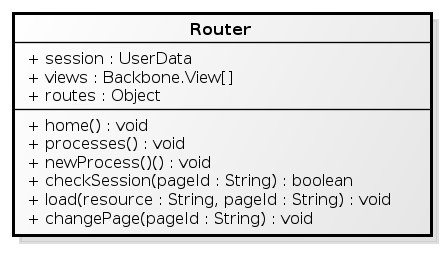
\includegraphics[width=%
\textwidth]
{./classi/client/presenter/Router.png} \caption{Diagramma classe \textit{Router}}
\end{figure}

\begin{flushleft}
\begin{itemize}
\item \textbf{Descrizione:} Classe che permette di coordinare l'inizializzazione e la renderizzazione delle pagine, gestendo gli eventi e le azioni di cambio pagina;
\item \textbf{Relazioni con altri componenti:}
\begin{sloppypar}
La classe reperisce le informazioni di sessione dalla classe \texttt{\model{}::U\fshyp{}ser\fshyp{}Mo\fshyp{}del} e comunica con le seguenti classi se l'utente dispone dei diritti d'accesso necessari:
\begin{itemize}
\item \texttt{\logic{}.Lo\fshyp{}gin};
\item \texttt{\logicUser{}.Re\fshyp{}gis\fshyp{}ter};
\item \texttt{\logicUser{}.Ma\fshyp{}in\fshyp{}Us\fshyp{}er};
\item \texttt{\logicUser{}.Us\fshyp{}er\fshyp{}Da\fshyp{}ta};
\item \texttt{\logicUser{}.Op\fshyp{}en\fshyp{}Pro\fshyp{}cess\fshyp{}gic};
\item \texttt{\logicUser{}.Ma\fshyp{}nag\fshyp{}ment\fshyp{}Pro\fshyp{}cess};
\item \texttt{\logicAdmin{}.Ma\fshyp{}in\fshyp{}Pro\fshyp{}cess\fshyp{}Ow\fshyp{}ner};
\item \texttt{\logicAdmin{}.O\fshyp{}pen\fshyp{}Pro\fshyp{}cess};
\item \texttt{\logicAdmin{}.New\fshyp{}Pro\fshyp{}cess};
\item \texttt{\logicAdmin{}.Check\fshyp{}Step};
\item \texttt{\logicAdmin{}.Ma\fshyp{}na\fshyp{}ge\fshyp{}Pro\fshyp{}cess};
\end{itemize}
\end{sloppypar}
\item \textbf{Attributi:}
\begin{sloppypar}
\begin{itemize}
\item \texttt{+ UserData session:}\\ oggetto di tipo \texttt{\model{}.U\fshyp{}ser\fshyp{}Da\fshyp{}ta}, che consente di gestire la sessione dell'utente;
\item \texttt{+ Backbone.View[] views:}\\ array che contiene le classi del presenter in esecuzione;
\item \texttt{+ Object routes:}\\ oggetto ridefinito da \texttt{Backbone.Router} che associa ad ogni evento di \textit{routing\ped{G}}, un metodo della classe;
\end{itemize}
\end{sloppypar}
\item \textbf{Metodi:}
\begin{sloppypar}
\begin{itemize}
\item \texttt{+ void home():}\\ gestisce l'evento di \textit{routing\ped{G} home};
\item \texttt{+ void processes():}\\ gestisce l'evento di \textit{routing\ped{G} processes};
\item \texttt{+ void newProcess():}\\ gestisce l'evento di \textit{routing\ped{G} newProcess};
\item \texttt{+ void checkStep():}\\ gestisce l'evento di \textit{routing\ped{G} checkStep};
\item \texttt{+ void process():}\\ gestisce l'evento di \textit{routing\ped{G} process};
\item \texttt{+ void register():}\\ gestisce l'evento di \textit{routing\ped{G} register};
\item \texttt{+ void user():}\\ gestisce l'evento di \textit{routing\ped{G} user};
\item \texttt{+ bool checkSession(String pageId):}\\ ritorna \texttt{true} solo se l'utente è autenticato; in caso contrario crea e renderizza la pagina di \textit{login};
\item \texttt{+ void load(String resource, String pageId):}\\ crea e aggiunge una vista di tipo \textit{resource} al campo dati \texttt{this.views}, all'indice \textit{pageId};
\item \texttt{+ void changePage(String pageId):}\\ imposta la pagina con id \textit{pageId} come attiva, ed esegue la transizione di cambio pagina.
\end{itemize}
\end{sloppypar}
\end{itemize}
\end{flushleft}

\paragraph{Login}
\label{login}

\begin{figure}[H] \centering 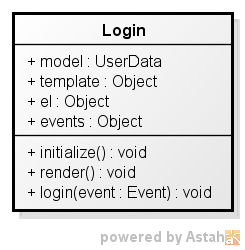
\includegraphics[width=%
\textwidth]
{./classi/client/presenter/Login.png} \caption{Diagramma classe  \textit{Login}}
\end{figure}

\begin{flushleft}
\begin{itemize}
\item \textbf{Descrizione:} Classe che ha il compito di gestire le richieste di autenticazione al sistema;
\item \textbf{Relazioni con altri componenti:}
\begin{sloppypar}
La classe gestisce i dati di sessione comunicando con la classe \texttt{\model{}.U\fshyp{}ser\fshyp{}Mo\fshyp{}del} e realizza l'interfaccia grafica utilizzando il \textit{template} \texttt{\view{}Lo\fshyp{}gin}.
\end{sloppypar}
\item \textbf{Attributi:}
\begin{sloppypar}
\begin{itemize}
\item \texttt{+ UserDataModel model:}\\ campo dati di tipo \texttt{\model{}.U\fshyp{}ser\fshyp{}Mo\fshyp{}del} che contiene i dati di sessione dell'utente;
\item \texttt{+ Object template:}\\ oggetto ridefinito da \texttt{Backbone.View}, che contiene il \textit{template HTML\ped{G}} associato alla classe;
\item \texttt{+ Object el:}\\ oggetto ridefinito da \texttt{Backbone.View} che rappresenta l'elemento \textit{HTML\ped{G}} entro cui la classe ascolta eventi generati dagli utenti;
\item \texttt{+ Object events:}\\ oggetto ridefinito da \texttt{Backbone.View} che associa ad ogni evento generato dagli utenti nella pagina \textit{HTML\ped{G}}, un metodo della classe;
\end{itemize}
\end{sloppypar}
\item \textbf{Metodi:}
\begin{sloppypar}
\begin{itemize}
\item \texttt{+ void initialize():}\\ metodo ridefinito da \texttt{Backbone.View}, invocato alla costruzione di ciascun oggetto della classe, che consente di aggiungere una pagina \textit{HTML\ped{G}} associata al componente;
\item \texttt{+ void render():}\\ metodo ridefinito da \texttt{Backbone.View}, che consente di aggiungere alla pagina \textit{HTML\ped{G}} il \textit{template} campo dati della classe;
\item \texttt{+ void login(Event event):}\\ effettua una richiesta di \textit{login}, utilizzando il campo dati \model{} per comunicare con il \textit{server\ped{G}}.
\end{itemize}
\end{sloppypar}
\end{itemize}
\end{flushleft}

\subsubsection{Package \logicUser{}}

\paragraph{MainUser}
\label{mainUser}

\begin{figure}[H] \centering 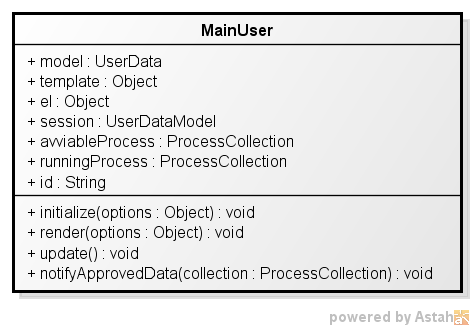
\includegraphics[width=%
\textwidth]
{./classi/client/presenter/user/MainUser.png} \caption{Diagramma classe  \textit{MainUser}}
\end{figure}

\begin{flushleft}
\begin{itemize}
\item \textbf{Descrizione:} Classe che ha il compito della gestione generale della logica delle funzionalità utente;
\item \textbf{Relazioni con altri componenti:}
\begin{sloppypar}
La classe comunica con l'interfaccia \texttt{\viewUser{}.I\fshyp{}Main\fshyp{}U\fshyp{}ser} per la realizzazione dell'interfaccia grafica.
\end{sloppypar}
\item \textbf{Attributi:}
\begin{sloppypar}
\begin{itemize}
\item \texttt{+ UserDataModel model:}\\ campo dati di tipo \texttt{\model{}.U\fshyp{}ser\fshyp{}Mo\fshyp{}del} che contiene i dati di sessione dell'utente;
\item \texttt{+ Object template:}\\ oggetto ridefinito da \texttt{Backbone.View}, che contiene il \textit{template HTML\ped{G}} associato alla classe;
\item \texttt{+ Object el:}\\ oggetto ridefinito da \texttt{Backbone.View} che rappresenta l'elemento \textit{HTML\ped{G}} entro cui la classe ascolta eventi generati dagli utenti;
\item \texttt{+ Object events:}\\ oggetto ridefinito da \texttt{Backbone.View} che associa ad ogni evento generato dagli utenti nella pagina \textit{HTML\ped{G}}, un metodo della classe;
\end{itemize}
\end{sloppypar}
\item \textbf{Metodi:}
\begin{sloppypar}
\begin{itemize}
\item \texttt{+ void initialize():}\\ metodo ridefinito da \texttt{Backbone.View}, invocato alla costruzione di ciascun oggetto della classe, che consente di aggiungere una pagina \textit{HTML\ped{G}} associata al componente;
\item \texttt{+ void render():}\\ metodo ridefinito da \texttt{Backbone.View}, che consente di aggiungere alla pagina \textit{HTML\ped{G}} il \textit{template} campo dati della classe.
\end{itemize}
\end{sloppypar}
\end{itemize}
\end{flushleft}

\paragraph{Register}
\label{register}

\begin{figure}[H] \centering 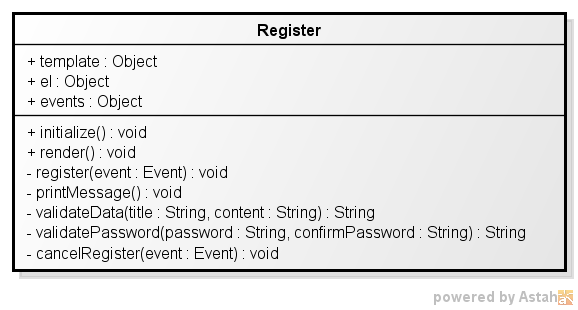
\includegraphics[width=%
\textwidth]
{./classi/client/presenter/user/Register.png} \caption{Diagramma classe  \textit{Register}}
\end{figure}

\begin{flushleft}
\begin{itemize}
\item \textbf{Descrizione:} Classe che ha il compito di gestire le richieste di registrazione da parte dell'utente;
\item \textbf{Relazioni con altri componenti:}
\begin{sloppypar}
La classe comunica con l'interfaccia \texttt{\viewUser{}.I\fshyp{}Re\fshyp{}gi\fshyp{}ster} per la realizzazione dei \textit{widget} per la registrazione, e con la classe \texttt{\model{}.U\fshyp{}ser\fshyp{}Mo\fshyp{}del} per comunicare col il \textit{server\ped{G}}.
\end{sloppypar}
\item \textbf{Attributi:}
\begin{sloppypar}
\begin{itemize}
\item \texttt{+ UserDataModel model:}\\ campo dati di tipo \texttt{\model{}.U\fshyp{}ser\fshyp{}Mo\fshyp{}del} che contiene i dati utente e di sessione;
\item \texttt{+ Object template:}\\ oggetto ridefinito da \texttt{Backbone.View}, che contiene il \textit{template HTML\ped{G}} associato alla classe;
\item \texttt{+ Object el:}\\ oggetto ridefinito da \texttt{Backbone.View} che rappresenta l'elemento \textit{HTML\ped{G}} entro cui la classe ascolta eventi generati dagli utenti;
\item \texttt{+ Object events:}\\ oggetto ridefinito da \texttt{Backbone.View} che associa ad ogni evento generato dagli utenti nella pagina \textit{HTML\ped{G}}, un metodo della classe;
\end{itemize}
\end{sloppypar}
\item \textbf{Metodi:}
\begin{sloppypar}
\begin{itemize}
\item \texttt{+ void initialize():}\\ metodo ridefinito da \texttt{Backbone.View}, invocato alla costruzione di ciascun oggetto della classe, che consente di aggiungere una pagina \textit{HTML\ped{G}} associata al componente;
\item \texttt{+ void render():}\\ metodo ridefinito da \texttt{Backbone.View}, che consente di aggiungere alla pagina \textit{HTML\ped{G}} il \textit{template} campo dati della classe;
\item \texttt{+ void register(Event event):}\\ effettua una richiesta di registrazione, utilizzando il campo dati \model{} per comunicare con il \textit{server\ped{G}}.
\end{itemize}
\end{sloppypar}
\end{itemize}
\end{flushleft}

\paragraph{UserData}
\label{userData}

\begin{figure}[H] \centering 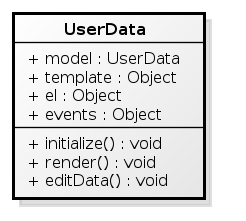
\includegraphics[width=%
\textwidth]
{./classi/client/presenter/user/UserData.png} \caption{Diagramma classe  \textit{UserData}}
\end{figure}

\begin{flushleft}
\begin{itemize}
\item \textbf{Descrizione:} Classe che ha il compito di gestire la visualizzazione e la modifica dei dati dell'utente;
\item \textbf{Relazioni con altri componenti:}
\begin{sloppypar}
La classe comunica con l'interfaccia \texttt{\viewUser{}.I\fshyp{}Us\fshyp{}er\fshyp{}Da\fshyp{}ta} per realizzare il \textit{widget} preposto alla visualizzazione e modifica dei dati dell'utente, e con la classe \texttt{\model{}.U\fshyp{}ser\fshyp{}Mo\fshyp{}del} per comunicare col il \textit{server\ped{G}}.
\end{sloppypar}
\item \textbf{Attributi:}
\begin{sloppypar}
\begin{itemize}
\item \texttt{+ UserDataModel model:}\\ campo dati di tipo \texttt{\model{}.U\fshyp{}ser\fshyp{}Mo\fshyp{}del} che contiene i dati utente e di sessione;
\item \texttt{+ Object template:}\\ oggetto ridefinito da \texttt{Backbone.View}, che contiene il \textit{template HTML\ped{G}} associato alla classe;
\item \texttt{+ Object el:}\\ oggetto ridefinito da \texttt{Backbone.View} che rappresenta l'elemento \textit{HTML\ped{G}} entro cui la classe ascolta eventi generati dagli utenti;
\item \texttt{+ Object events:}\\ oggetto ridefinito da \texttt{Backbone.View} che associa ad ogni evento generato dagli utenti nella pagina \textit{HTML\ped{G}}, un metodo della classe;
\end{itemize}
\end{sloppypar}
\item \textbf{Metodi:}
\begin{sloppypar}
\begin{itemize}
\item \texttt{+ void initialize():}\\ metodo ridefinito da \texttt{Backbone.View}, invocato alla costruzione di ciascun oggetto della classe, che consente di aggiungere una pagina \textit{HTML\ped{G}} associata al componente;
\item \texttt{+ void render():}\\ metodo ridefinito da \texttt{Backbone.View}, che consente di aggiungere alla pagina \textit{HTML\ped{G}} il \textit{template} campo dati della classe;
\item \texttt{+ void editData():}\\ utilizza il campo dati \texttt{model} per salvare i dati modificati dall'utente nel \textit{server\ped{G}}.
\end{itemize}
\end{sloppypar}
\end{itemize}
\end{flushleft}

\paragraph{OpenProcess}
\label{openProcessU}

\begin{figure}[H] \centering 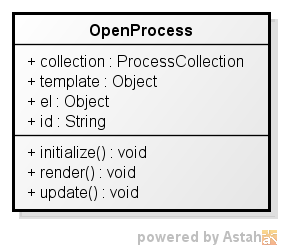
\includegraphics[width=%
\textwidth]
{./classi/client/presenter/user/OpenProcess.png} \caption{Diagramma classe  \textit{OpenProcess}}
\end{figure}

\begin{flushleft}
\begin{itemize}
\item \textbf{Descrizione:} Classe che ha il compito di selezionare, ricercare e aprire un processo fra quelli eseguibili;
\item \textbf{Relazioni con altri componenti:}
\begin{sloppypar}
La classe realizza e modifica l'opportuno \textit{widget} mediante l'interfaccia \texttt{\viewUser{}.I\fshyp{}Op\fshyp{}en\fshyp{}Pro\fshyp{}cess} e utilizza la classe \texttt{\collection{}.Pro\fshyp{}cess\fshyp{}Col\fshyp{}lec\fshyp{}tion} per gestire e ottenere i dati dal \textit{server\ped{G}}.
\end{sloppypar}
\item \textbf{Attributi:}
\begin{sloppypar}
\begin{itemize}
\item \texttt{+ ProcessCollection collection:}\\ campo dati di tipo \texttt{\collection{}.Pro\fshyp{}cess\fshyp{}Col\fshyp{}lec\fshyp{}tion} che contiene la lista dei processi non terminati o non ancora eliminati dall'utente;
\item \texttt{+ Object template:}\\ oggetto ridefinito da \texttt{Backbone.View}, che contiene il \textit{template HTML\ped{G}} associato alla classe;
\item \texttt{+ Object el:}\\ oggetto ridefinito da \texttt{Backbone.View} che rappresenta l'elemento \textit{HTML\ped{G}} entro cui la classe ascolta eventi generati dagli utenti;
\item \texttt{+ String id:}\\ campo dati ridefinito da \texttt{Backbone.View} contente l'id della classe;
\end{itemize}
\end{sloppypar}
\item \textbf{Metodi:}
\begin{sloppypar}
\begin{itemize}
\item \texttt{+ void initialize():}\\ metodo ridefinito da \texttt{Backbone.View}, invocato alla costruzione di ciascun oggetto della classe, che consente di aggiungere una pagina \textit{HTML\ped{G}} associata al componente;
\item \texttt{+ void render():}\\ metodo ridefinito da \texttt{Backbone.View}, che consente di aggiungere alla pagina \textit{HTML\ped{G}} il \textit{template} campo dati della classe;
\item \texttt{+ void update():}\\ aggiorna il campo dati \texttt{collection} comunicando con il \textit{server\ped{G}}.
\end{itemize}
\end{sloppypar}
\end{itemize}
\end{flushleft}

\paragraph{ManagementProcess}
\label{managementProcessU}
\begin{flushleft}

\begin{figure}[H] \centering 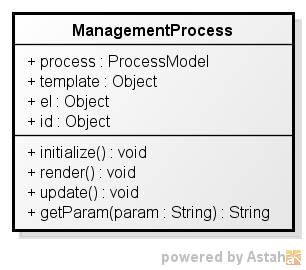
\includegraphics[width=%
\textwidth]
{./classi/client/presenter/user/ManagementProcess.png} \caption{Diagramma classe  \textit{ManagementProcess}}
\end{figure}

\begin{itemize}
\item \textbf{Descrizione:} Classe che ha il compito di gestire e accedere alle informazioni relative allo stato del processo selezionato.;
\item \textbf{Relazioni con altri componenti:}
\begin{sloppypar}
La classe comunica con l'interfaccia \texttt{\viewUser{}.I\fshyp{}Ma\fshyp{}na\fshyp{}gment\fshyp{}Pro\fshyp{}cess} per realizzare il \textit{widget} che permette la gestione del processo selezionato, utilizza la classe \texttt{\model{}.Pro\fshyp{}cess\fshyp{}Mo\fshyp{}del} per gestire e ottenere i dati dal \textit{server\ped{G}}, e provvede ad invocare le seguenti classi in base alle decisioni dell'utente:
\begin{itemize}
\item \texttt{\logicUser{}.Print\fshyp{}Re\fshyp{}port};
\item \texttt{\logicUser{}.Send\fshyp{}Da\fshyp{}ta}.
\end{itemize}
\end{sloppypar}
\item \textbf{Attributi:}
\begin{sloppypar}
\begin{itemize}
\item \texttt{+ ProcessModel process:}\\ campo dati di tipo \texttt{\model{}.Pro\fshyp{}cess\fshyp{}Mo\fshyp{}del} che contiene i dati del processo in gestione;
\item \texttt{+ Object template:}\\ oggetto ridefinito da \texttt{Backbone.View}, che contiene il \textit{template HTML\ped{G}} associato alla classe;
\item \texttt{+ Object el:}\\ oggetto ridefinito da \texttt{Backbone.View} che rappresenta l'elemento \textit{HTML\ped{G}} entro cui la classe ascolta eventi generati dagli utenti;
\item \texttt{+ String id:}\\ campo dati ridefinito da \texttt{Backbone.View} contente l'id della classe;
\end{itemize}
\end{sloppypar}
\item \textbf{Metodi:}
\begin{sloppypar}
\begin{itemize}
\item \texttt{+ void initialize():}\\ metodo ridefinito da \texttt{Backbone.View}, invocato alla costruzione di ciascun oggetto della classe, che consente di aggiungere una pagina \textit{HTML\ped{G}} associata al componente;
\item \texttt{+ void render():}\\ metodo ridefinito da \texttt{Backbone.View}, che consente di aggiungere alla pagina \textit{HTML\ped{G}} il \textit{template} campo dati della classe;
\item \texttt{+ void update():}\\ aggiorna i campi dati \texttt{process} e \texttt{processData} comunicando con il \textit{server\ped{G}};
\item \texttt{+ String getParam(String param):}\\ ritorna il valore del parametro \textit{param} se presente nella \textit{URL\ped{G}}.
\end{itemize}
\end{sloppypar}
\end{itemize}
\end{flushleft}

\paragraph{PrintReport}
\label{printReport}

\begin{figure}[H] \centering 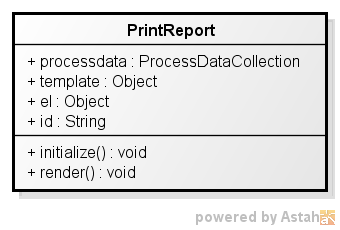
\includegraphics[width=%
\textwidth]
{./classi/client/presenter/user/PrintReport.png} \caption{Diagramma classe  \textit{PrintReport}}
\end{figure}

\begin{flushleft}
\begin{itemize}
\item \textbf{Descrizione:} Classe che ha il compito di gestire la creazione del report di fine processo;
\item \textbf{Relazioni con altri componenti:}
\begin{sloppypar}
La classe comunica con l'interfaccia \texttt{\viewUser{}.I\fshyp{}Print\fshyp{}Re\fshyp{}port} per realizzare il \textit{widget} per creare il report di fine processo, e utilizza la classe \texttt{\collection{}.Pro\fshyp{}cess\fshyp{}Data\fshyp{}Col\fshyp{}lec\fshyp{}tion} per gestire e ottenere i dati dal \textit{server\ped{G}}.
\end{sloppypar}
\item \textbf{Attributi:}
\begin{sloppypar}
\begin{itemize}
\item \texttt{+ ProcessDataCollection processdata:}\\ campo dati di tipo \texttt{\collection{}.Pro\fshyp{}cess\fshyp{}Da\fshyp{}ta\fshyp{}Col\fshyp{}lec\fshyp{}tion} che contiene i dati inviati dall'utente relativi al processo in gestione;
\item \texttt{+ Object template:}\\ oggetto ridefinito da \texttt{Backbone.View}, che contiene il \textit{template HTML\ped{G}} associato alla classe;
\item \texttt{+ Object el:}\\ oggetto ridefinito da \texttt{Backbone.View} che rappresenta l'elemento \textit{HTML\ped{G}} entro cui la classe ascolta eventi generati dagli utenti;
\item \texttt{+ String id:}\\ campo dati ridefinito da \texttt{Backbone.View} contente l'id della classe;
\end{itemize}
\end{sloppypar}
\item \textbf{Metodi:}
\begin{sloppypar}
\begin{itemize}
\item \texttt{+ void initialize():}\\ metodo ridefinito da \texttt{Backbone.View}, invocato alla costruzione di ciascun oggetto della classe, che consente di aggiungere una pagina \textit{HTML\ped{G}} associata al componente;
\item \texttt{+ void render():}\\ metodo ridefinito da \texttt{Backbone.View}, che consente di aggiungere alla pagina \textit{HTML\ped{G}} il \textit{template} campo dati della classe.
\end{itemize}
\end{sloppypar}
\end{itemize}
\end{flushleft}

\paragraph{SendData}
\label{sendData}

\begin{figure}[H] \centering 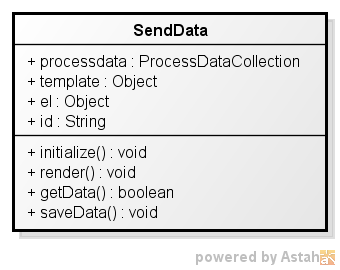
\includegraphics[width=%
\textwidth]
{./classi/client/presenter/user/SendData.png} \caption{Diagramma classe  \textit{SendData}}
\end{figure}

\begin{flushleft}
\begin{itemize}
\item \textbf{Descrizione:} Classe che ha il compito di gestire l'inserimento e l'invio di dati da parte degli utenti, per completare il passo corrente;
\item \textbf{Relazioni con altri componenti:}
\begin{sloppypar}
La classe comunica con l'interfaccia \texttt{\viewUser{}.I\fshyp{}Send\fshyp{}Da\fshyp{}ta} per creare il \textit{widget} che consente di inviare i dati, utilizza la classe \texttt{\collection{}.Pro\fshyp{}cess\fshyp{}Data\fshyp{}Col\fshyp{}lec\fshyp{}tion} per gestire e ottenere i dati dal \textit{server\ped{G}}, e infine invoca le seguenti classi che gestiscono l'invio di un tipo di dato specifico:
\begin{itemize}
	\item \texttt{\logicUser{}.SendText};
	\item \texttt{\logicUser{}.SendNumb};
	\item \texttt{\logicUser{}.SendImage};
	\item \texttt{\logicUser{}.SendPosition}.
\end{itemize}
\end{sloppypar}
\item \textbf{Attributi:}
\begin{sloppypar}
\begin{itemize}
\item \texttt{+ ProcessDataCollection processdata:}\\ campo dati di tipo \texttt{\collection{}.Pro\fshyp{}cess\fshyp{}Da\fshyp{}ta\fshyp{}Col\fshyp{}lec\fshyp{}tion} che consente di interagire con la lista dei dati inviati dall'utente relativa al processo in gestione presente nel \textit{server\ped{G}};
\item \texttt{+ Object template:}\\ oggetto ridefinito da \texttt{Backbone.View}, che contiene il \textit{template HTML\ped{G}} associato alla classe;
\item \texttt{+ Object el:}\\ oggetto ridefinito da \texttt{Backbone.View} che rappresenta l'elemento \textit{HTML\ped{G}} entro cui la classe ascolta eventi generati dagli utenti;
\item \texttt{+ String id:}\\ campo dati ridefinito da \texttt{Backbone.View} contente l'id della classe;
\end{itemize}
\end{sloppypar}
\item \textbf{Metodi:}
\begin{sloppypar}
\begin{itemize}
\item \texttt{+ void initialize():}\\ metodo ridefinito da \texttt{Backbone.View}, invocato alla costruzione di ciascun oggetto della classe, che consente di aggiungere una pagina \textit{HTML\ped{G}} associata al componente;
\item \texttt{+ void render():}\\ metodo ridefinito da \texttt{Backbone.View}, che consente di aggiungere alla pagina \textit{HTML\ped{G}} il \textit{template} campo dati della classe. Utilizza le classi \texttt{\logicUser{}.SendText} \texttt{\logicUser{}.SendNumb}, \texttt{\logicUser{}.SendImage} e \texttt{\logicUser{}.SendPosition} per renderizzare l'interfaccia relativa all'inserimento dei diversi tipi di dato;
\item \texttt{+ bool getData():}\\ controlla se i dati inseriti dall'utente sono corretti: se lo sono ritorna \texttt{true} e li aggiunge alla collezione \texttt{processData}, altrimenti ritorna \texttt{false};
\item \texttt{+ bool saveData():}\\ utilizza metodi del campo dati \texttt{processData}, per inviare i dati raccolti al \textit{server\ped{G}}.
\end{itemize}
\end{sloppypar}
\end{itemize}
\end{flushleft}

\paragraph{SendText}
\label{sendText}

\begin{figure}[H] \centering 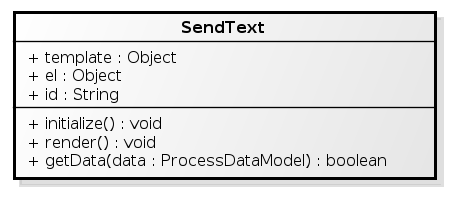
\includegraphics[width=%
\textwidth]
{./classi/client/presenter/user/SendText.png} \caption{Diagramma classe  \textit{SendText}}
\end{figure}

\begin{flushleft}
\begin{itemize}
\item \textbf{Descrizione:} Classe che permette l'inserimento e il controllo di dati testuali inseriti dagli utenti;
\item \textbf{Relazioni con altri componenti:}
\begin{sloppypar}
La classe, mediante l'interfaccia \texttt{\viewUser{}.I\fshyp{}Send\fshyp{}Text}, realizza e aggiorna l'opportuno \textit{widget}.
\end{sloppypar}
\item \textbf{Attributi:}
\begin{sloppypar}
\begin{itemize}
\item \texttt{+ Object template:}\\ oggetto ridefinito da \texttt{Backbone.View}, che contiene il \textit{template HTML\ped{G}} associato alla classe;
\item \texttt{+ Object el:}\\ oggetto ridefinito da \texttt{Backbone.View} che rappresenta l'elemento \textit{HTML\ped{G}} entro cui la classe ascolta eventi generati dagli utenti;
\item \texttt{+ String id:}\\ campo dati ridefinito da \texttt{Backbone.View} contente l'id della classe;
\end{itemize}
\end{sloppypar}
\item \textbf{Metodi:}
\begin{sloppypar}
\begin{itemize}
\item \texttt{+ void initialize():}\\ metodo ridefinito da \texttt{Backbone.View}, invocato alla costruzione di ciascun oggetto della classe, che consente di aggiungere una pagina \textit{HTML\ped{G}} associata al componente;
\item \texttt{+ void render():}\\ metodo ridefinito da \texttt{Backbone.View}, che consente di aggiungere alla pagina \textit{HTML\ped{G}} il \textit{template} campo dati della classe;
\item \texttt{+ bool getData(ProcessDataModel data):}\\ controlla se i dati inseriti dall'utente sono corretti: se lo sono ritorna \texttt{true} e li aggiunge al riferimento \texttt{data}, altrimenti ritorna \texttt{false}.
\end{itemize}
\end{sloppypar}
\end{itemize}
\end{flushleft}

\paragraph{SendNumb}
\label{sendNumb}

\begin{figure}[H] \centering 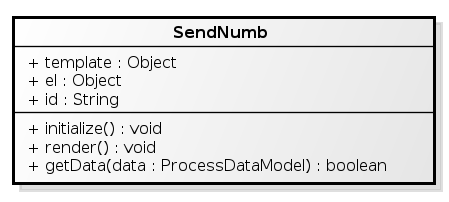
\includegraphics[width=%
\textwidth]
{./classi/client/presenter/user/SendNumb.png} \caption{Diagramma classe  \textit{SendNumb}}
\end{figure}

\begin{flushleft}
\begin{itemize}
\item \textbf{Descrizione:} Classe che ha il compito di permettere l'inserimento e il controllo di dati numerici inseriti dagli utenti;
\item \textbf{Relazioni con altri componenti:}
\begin{sloppypar}
La classe, mediante l'interfaccia \texttt{\viewUser{}.I\fshyp{}Send\fshyp{}Numb}, realizza e aggiorna l'opportuno \textit{widget}.
\end{sloppypar}
\item \textbf{Attributi:}
\begin{sloppypar}
\begin{itemize}
\item \texttt{+ Object template:}\\ oggetto ridefinito da \texttt{Backbone.View}, che contiene il \textit{template HTML\ped{G}} associato alla classe;
\item \texttt{+ Object el:}\\ oggetto ridefinito da \texttt{Backbone.View} che rappresenta l'elemento \textit{HTML\ped{G}} entro cui la classe ascolta eventi generati dagli utenti;
\item \texttt{+ String id:}\\ campo dati ridefinito da \texttt{Backbone.View} contente l'id della classe;
\end{itemize}
\end{sloppypar}
\item \textbf{Metodi:}
\begin{sloppypar}
\begin{itemize}
\item \texttt{+ void initialize():}\\ metodo ridefinito da \texttt{Backbone.View}, invocato alla costruzione di ciascun oggetto della classe, che consente di aggiungere una pagina \textit{HTML\ped{G}} associata al componente;
\item \texttt{+ void render():}\\ metodo ridefinito da \texttt{Backbone.View}, che consente di aggiungere alla pagina \textit{HTML\ped{G}} il \textit{template} campo dati della classe;
\item \texttt{+ bool getData(ProcessDataModel data):}\\ controlla se i dati inseriti dall'utente sono corretti: se lo sono ritorna \texttt{true} e li aggiunge al riferimento \texttt{data}, altrimenti ritorna \texttt{false}.
\end{itemize}
\end{sloppypar}
\end{itemize}
\end{flushleft}

\paragraph{SendImage}
\label{sendImage}

\begin{figure}[H] \centering 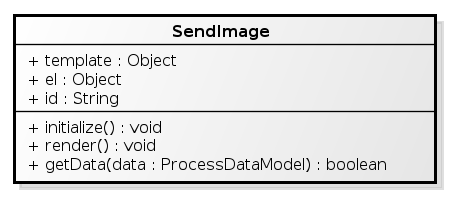
\includegraphics[width=%
\textwidth]
{./classi/client/presenter/user/SendImage.png} \caption{Diagramma classe  \textit{SendImage}}
\end{figure}

\begin{flushleft}
\begin{itemize}
\item \textbf{Descrizione:} Classe che gestisce l'inserimento e il controllo di immagini inserite dagli degli utenti;
\item \textbf{Relazioni con altri componenti:}
\begin{sloppypar}
La classe, mediante l'interfaccia \texttt{\viewUser{}.I\fshyp{}Send\fshyp{}Ima\fshyp{}ge}, realizza e aggiorna l'opportuno \textit{widget}.
\end{sloppypar}
\item \textbf{Attributi:}
\begin{sloppypar}
\begin{itemize}
\item \texttt{+ Object template:}\\ oggetto ridefinito da \texttt{Backbone.View}, che contiene il \textit{template HTML\ped{G}} associato alla classe;
\item \texttt{+ Object el:}\\ oggetto ridefinito da \texttt{Backbone.View} che rappresenta l'elemento \textit{HTML\ped{G}} entro cui la classe ascolta eventi generati dagli utenti;
\item \texttt{+ String id:}\\ campo dati ridefinito da \texttt{Backbone.View} contente l'id della classe;
\end{itemize}
\end{sloppypar}
\item \textbf{Metodi:}
\begin{sloppypar}
\begin{itemize}
\item \texttt{+ void initialize():}\\ metodo ridefinito da \texttt{Backbone.View}, invocato alla costruzione di ciascun oggetto della classe, che consente di aggiungere una pagina \textit{HTML\ped{G}} associata al componente;
\item \texttt{+ void render():}\\ metodo ridefinito da \texttt{Backbone.View}, che consente di aggiungere alla pagina \textit{HTML\ped{G}} il \textit{template} campo dati della classe;
\item \texttt{+ bool getData(ProcessDataModel data):}\\ controlla se i dati inseriti dall'utente sono corretti: se lo sono ritorna \texttt{true} e li aggiunge al riferimento \texttt{data}, altrimenti ritorna \texttt{false}.
\end{itemize}
\end{sloppypar}
\end{itemize}
\end{flushleft}

\paragraph{SendPosition}
\label{sendPosition}

\begin{figure}[H] \centering 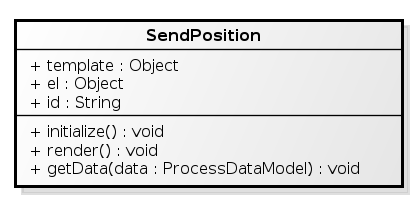
\includegraphics[width=%
\textwidth]
{./classi/client/presenter/user/SendPosition.png} \caption{Diagramma classe  \textit{SendPosition}}
\end{figure}

\begin{flushleft}
\begin{itemize}
\item \textbf{Descrizione:} Classe che ha il compito di gestire il calcolo e il controllo della posizione geografica dell'utente;
\item \textbf{Relazioni con altri componenti:}
\begin{sloppypar}
La classe, mediante l'interfaccia \texttt{\viewUser{}.I\fshyp{}Send\fshyp{}Po\fshyp{}si\fshyp{}tion}, realizza e aggiorna l'opportuno \textit{widget}.
\end{sloppypar}
\item \textbf{Attributi:}
\begin{sloppypar}
\begin{itemize}
\item \texttt{+ Object template:}\\ oggetto ridefinito da \texttt{Backbone.View}, che contiene il \textit{template HTML\ped{G}} associato alla classe;
\item \texttt{+ Object el:}\\ oggetto ridefinito da \texttt{Backbone.View} che rappresenta l'elemento \textit{HTML\ped{G}} entro cui la classe ascolta eventi generati dagli utenti;
\item \texttt{+ String id:}\\ campo dati ridefinito da \texttt{Backbone.View} contente l'id della classe;
\end{itemize}
\end{sloppypar}
\item \textbf{Metodi:}
\begin{sloppypar}
\begin{itemize}
\item \texttt{+ void initialize():}\\ metodo ridefinito da \texttt{Backbone.View}, invocato alla costruzione di ciascun oggetto della classe, che consente di aggiungere una pagina \textit{HTML\ped{G}} associata al componente;
\item \texttt{+ void render():}\\ metodo ridefinito da \texttt{Backbone.View}, che consente di aggiungere alla pagina \textit{HTML\ped{G}} il \textit{template} campo dati della classe;
\item \texttt{+ bool getData(ProcessDataModel data):}\\ controlla se i dati inseriti dall'utente sono corretti: se lo sono ritorna \texttt{true} e li aggiunge al riferimento \texttt{data}, altrimenti ritorna \texttt{false}.
\end{itemize}
\end{sloppypar}
\end{itemize}
\end{flushleft}

\subsubsection{Package \logicAdmin{}}

\paragraph{MainProcessOwner}
\label{mainProcessOwner}

\begin{figure}[H] \centering 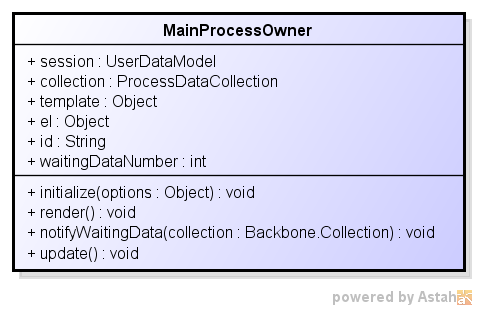
\includegraphics[width=%
\textwidth]
{./classi/client/presenter/po/MainProcessOwner.png} \caption{Diagramma classe  \textit{MainProcessOwner}}
\end{figure}

\begin{flushleft}
\begin{itemize}
\item \textbf{Descrizione:} Classe che ha il compito della gestione generale della logica delle funzionalità \textit{Process Owner\ped{G}};
\item \textbf{Relazioni con altri componenti:}
\begin{sloppypar}
La classe comunica con il \textit{template} \texttt{\viewAdmin{}.I\fshyp{}Main\fshyp{}Pro\fshyp{}cess\fshyp{}Ow\fshyp{}ner} per la realizzazione dell'interfaccia grafica.
\end{sloppypar}
\item \textbf{Attributi:}
\begin{sloppypar}
\begin{itemize}
\item \texttt{+ Object template:}\\ oggetto ridefinito da \texttt{Backbone.View}, che contiene il \textit{template HTML\ped{G}} associato alla classe;
\item \texttt{+ Object el:}\\ oggetto ridefinito da \texttt{Backbone.View} che rappresenta l'elemento \textit{HTML\ped{G}} entro cui la classe ascolta eventi generati dagli utenti;
\item \texttt{+ String id:}\\ campo dati ridefinito da \texttt{Backbone.View} contente l'id della classe;
\end{itemize}
\end{sloppypar}
\item \textbf{Metodi:}
\begin{sloppypar}
\begin{itemize}
\item \texttt{+ void initialize():}\\ metodo ridefinito da \texttt{Backbone.View}, invocato alla costruzione di ciascun oggetto della classe, che consente di aggiungere una pagina \textit{HTML\ped{G}} associata al componente;
\item \texttt{+ void render():}\\ metodo ridefinito da \texttt{Backbone.View}, che consente di aggiungere alla pagina \textit{HTML\ped{G}} il \textit{template} campo dati della classe.
\end{itemize}
\end{sloppypar}
\end{itemize}
\end{flushleft}

\paragraph{OpenProcess}
\label{openProcess}

\begin{figure}[H] \centering 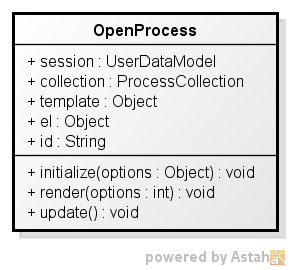
\includegraphics[width=%
\textwidth]
{./classi/client/presenter/po/OpenProcess.png} \caption{Diagramma classe  \textit{OpenProcess}}
\end{figure}

\begin{flushleft}
\begin{itemize}
\item \textbf{Descrizione:} Classe che ha il compito di gestire la ricerca e la selezione di un processo;
\item \textbf{Relazioni con altri componenti:}
\begin{sloppypar}
La classe comunica con il \textit{template} \texttt{\viewAdmin{}.I\fshyp{}O\fshyp{}pen\fshyp{}Pro\fshyp{}cess} per la realizzazione dell'interfaccia grafica, e con la classe \texttt{\collection{}Pro\fshyp{}cess\fshyp{}Col\fshyp{}lec\fshyp{}tion} per gestire e ottenere i dati dal \textit{server\ped{G}}.
\end{sloppypar}
\item \textbf{Attributi:}
\begin{sloppypar}
\begin{itemize}
\item \texttt{+ ProcessCollection collection:}\\ campo dati di tipo \texttt{\collection{}.Pro\fshyp{}cess\fshyp{}Col\fshyp{}lec\fshyp{}tion} che contiene la lista dei processi non eliminati dal \textit{process owner\ped{G}};
\item \texttt{+ Object template:}\\ oggetto ridefinito da \texttt{Backbone.View}, che contiene il \textit{template HTML\ped{G}} associato alla classe;
\item \texttt{+ Object el:}\\ oggetto ridefinito da \texttt{Backbone.View} che rappresenta l'elemento \textit{HTML\ped{G}} entro cui la classe ascolta eventi generati dagli utenti;
\item \texttt{+ String id:}\\ campo dati ridefinito da \texttt{Backbone.View} contente l'id della classe;
\end{itemize}
\end{sloppypar}
\item \textbf{Metodi:}
\begin{sloppypar}
\begin{itemize}
\item \texttt{+ void initialize():}\\ metodo ridefinito da \texttt{Backbone.View}, invocato alla costruzione di ciascun oggetto della classe, che consente di aggiungere una pagina \textit{HTML\ped{G}} associata al componente;
\item \texttt{+ void render():}\\ metodo ridefinito da \texttt{Backbone.View}, che consente di aggiungere alla pagina \textit{HTML\ped{G}} il \textit{template} campo dati della classe;
\item \texttt{+ void update():}\\ aggiorna il campo dati \texttt{collection} comunicando con il \textit{server\ped{G}}.
\end{itemize}
\end{sloppypar}
\end{itemize}
\end{flushleft}

\paragraph{NewProcess}
\label{newProcess}
\begin{figure}[H] \centering 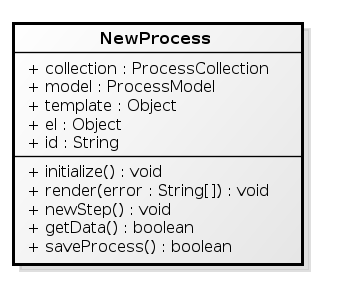
\includegraphics[width=%
\textwidth]
{./classi/client/presenter/po/NewProcess.png} \caption{Diagramma classe  \textit{NewProcess}}
\end{figure}

\begin{flushleft}
\begin{itemize}
\item \textbf{Descrizione:} Classe che ha il compito di gestire la logica della definizione di un nuovo processo;
\item \textbf{Relazioni con altri componenti:}
\begin{sloppypar}
La classe comunica con il \textit{template} \texttt{\viewAdmin{}.I\fshyp{}New\fshyp{}pro\fshyp{}cess} per la realizzazione dell'interfaccia grafica, con la classe \texttt{\collection{}.Pro\fshyp{}cess\fshyp{}Col\fshyp{}lec\fshyp{}tion} comunicare con il \textit{server\ped{G}} e con la classe \texttt{\logicAdmin{}.Add\fshyp{}Step};
\end{sloppypar}
\item \textbf{Attributi:}
\begin{sloppypar}
\begin{itemize}
\item \texttt{+ ProcessCollection collection:}\\ campo dati di tipo \texttt{\collection{}.Pro\fshyp{}cess\fshyp{}Col\fshyp{}lec\fshyp{}tion} che consente di interagire con la lista dei processi non eliminati dal \textit{process owner\ped{G}}, presente nel \textit{server\ped{G}};
\item \texttt{+ ProcessModel model:}\\ campo dati di tipo \texttt{\model{}.Pro\fshyp{}cess\fshyp{}Mo\fshyp{}del} che contiene i dati del processo in definizione;
\item \texttt{+ Object template:}\\ oggetto ridefinito da \texttt{Backbone.View}, che contiene il \textit{template HTML\ped{G}} associato alla classe;
\item \texttt{+ Object el:}\\ oggetto ridefinito da \texttt{Backbone.View} che rappresenta l'elemento \textit{HTML\ped{G}} entro cui la classe ascolta eventi generati dagli utenti;
\item \texttt{+ String id:}\\ campo dati ridefinito da \texttt{Backbone.View} contente l'id della classe;
\end{itemize}
\end{sloppypar}
\item \textbf{Metodi:}
\begin{sloppypar}
\begin{itemize}
\item \texttt{+ void initialize():}\\ metodo ridefinito da \texttt{Backbone.View}, invocato alla costruzione di ciascun oggetto della classe, che consente di aggiungere una pagina \textit{HTML\ped{G}} associata al componente;
\item \texttt{+ void render(String[] errors):}\\ metodo ridefinito da \texttt{Backbone.View}, che consente di aggiungere alla pagina \textit{HTML\ped{G}} il \textit{template} campo dati della classe, compilato con gli eventuali errori \texttt{errors};
\item \texttt{+ void newStep():}\\ utilizza la classe \texttt{\logicAdmin{}.Add\fshyp{}Step} per definire e aggiungere un nuovo passo al processo \texttt{model};
\item \texttt{+ bool getData():}\\ controlla se i dati inseriti dal \textit{process owner\ped{G}} sono corretti: se lo sono ritorna \texttt{true} e li aggiunge al processo \texttt{model}, altrimenti ritorna \texttt{false};
\item \texttt{+ bool saveProcess():}\\ utilizza metodi del campo dati \texttt{collection}, per inviare il processo \texttt{model} al \textit{server\ped{G}}.
\end{itemize}
\end{sloppypar}
\end{itemize}
\end{flushleft}

\paragraph{AddStep}
\label{addStep}

\begin{figure}[H] \centering 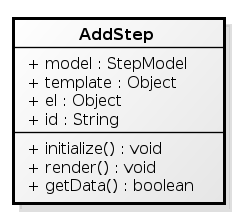
\includegraphics[width=%
\textwidth]
{./classi/client/presenter/po/AddStep.png} \caption{Diagramma classe  \textit{AddStep}}
\end{figure}

\begin{flushleft}
\begin{itemize}
\item \textbf{Descrizione:} Classe che ha il compito di gestire la logica di definizione dei passi di un processo;
\item \textbf{Relazioni con altri componenti:}
\begin{sloppypar}
La classe comunica con il \textit{template} \texttt{\viewAdmin{}.I\fshyp{}Add\fshyp{}Step} per la realizzazione dell'interfaccia grafica e utilizza la classe \texttt{\model{}.Step} per salvare i dati del passo in creazione.
\end{sloppypar}
\item \textbf{Attributi:}
\begin{sloppypar}
\begin{itemize}
\item \texttt{+ StepModel model:}\\ campo dati di tipo \texttt{\model{}.Step\fshyp{}Mo\fshyp{}del} che contiene i dati del passo in definizione;
\item \texttt{+ Object template:}\\ oggetto ridefinito da \texttt{Backbone.View}, che contiene il \textit{template HTML\ped{G}} associato alla classe;
\item \texttt{+ Object el:}\\ oggetto ridefinito da \texttt{Backbone.View} che rappresenta l'elemento \textit{HTML\ped{G}} entro cui la classe ascolta eventi generati dagli utenti;
\item \texttt{+ String id:}\\ campo dati ridefinito da \texttt{Backbone.View} contente l'id della classe;
\end{itemize}
\end{sloppypar}
\item \textbf{Metodi:}
\begin{sloppypar}
\begin{itemize}
\item \texttt{+ void initialize():}\\ metodo ridefinito da \texttt{Backbone.View}, invocato alla costruzione di ciascun oggetto della classe, che consente di aggiungere una pagina \textit{HTML\ped{G}} associata al componente;
\item \texttt{+ void render(String[] errors):}\\ metodo ridefinito da \texttt{Backbone.View}, che consente di aggiungere alla pagina \textit{HTML\ped{G}} il \textit{template} campo dati della classe, compilato con gli eventuali errori \texttt{errors};
\item \texttt{+ bool getData():}\\ controlla se i dati inseriti dal \textit{process owner\ped{G}} sono corretti: se lo sono ritorna \texttt{true} e li aggiunge al passo \texttt{model}, altrimenti ritorna \texttt{false}.
\end{itemize}
\end{sloppypar}
\end{itemize}
\end{flushleft}

\paragraph{ManageProcess}
\label{manageProcess}
\begin{figure}[H] \centering 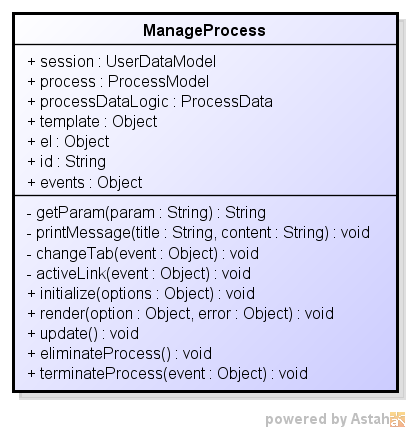
\includegraphics[width=%
\textwidth]
{./classi/client/presenter/po/ManageProcess.png} \caption{Diagramma classe  \textit{ManageProcess}}
\end{figure}
\begin{flushleft}
\begin{itemize}
\item \textbf{Descrizione:} Classe che ha il compito di gestire e accedere alle informazioni relative allo stato dei processi e ai dati inviati dagli utenti. Le operazioni di gestione dello stato comprendono la terminazione e l'eliminazione di un processo;
\item \textbf{Relazioni con altri componenti:}
\begin{sloppypar}
La classe comunica con il \textit{template} \texttt{\viewAdmin{}.I\fshyp{}Ma\fshyp{}na\fshyp{}ge\fshyp{}Pro\fshyp{}cess} per la realizzazione dell'interfaccia grafica, e con le classi \texttt{\collection{}.Pro\fshyp{}cess\fshyp{}Da\fshyp{}ta\fshyp{}Col\fshyp{}lec\fshyp{}tion} e \texttt{\model{}.Pro\fshyp{}cess\fshyp{}Mo\fshyp{}del} per gestire e ottenere i dati dal \textit{server\ped{G}}.
\end{sloppypar}
\item \textbf{Attributi:}
\begin{sloppypar}
\begin{itemize}
\item \texttt{+ ProcessModel process:}\\ campo dati di tipo \texttt{\model{}.Pro\fshyp{}cess\fshyp{}Mo\fshyp{}del} che contiene i dati del processo in gestione;
\item \texttt{+ ProcessDataCollection processdata:}\\ campo dati di tipo \texttt{\collection{}.Pro\fshyp{}cess\fshyp{}Da\fshyp{}ta\fshyp{}Col\fshyp{}lec\fshyp{}tion} che contiene i dati inviati dagli utenti relativi al processo in gestione;
\item \texttt{+ Object template:}\\ oggetto ridefinito da \texttt{Backbone.View}, che contiene il \textit{template HTML\ped{G}} associato alla classe;
\item \texttt{+ Object el:}\\ oggetto ridefinito da \texttt{Backbone.View} che rappresenta l'elemento \textit{HTML\ped{G}} entro cui la classe ascolta eventi generati dagli utenti;
\item \texttt{+ String id:}\\ campo dati ridefinito da \texttt{Backbone.View} contente l'id della classe;
\end{itemize}
\end{sloppypar}
\item \textbf{Metodi:}
\begin{sloppypar}
\begin{itemize}
\item \texttt{+ void initialize():}\\ metodo ridefinito da \texttt{Backbone.View}, invocato alla costruzione di ciascun oggetto della classe, che consente di aggiungere una pagina \textit{HTML\ped{G}} associata al componente;
\item \texttt{+ void render():}\\ metodo ridefinito da \texttt{Backbone.View}, che consente di aggiungere alla pagina \textit{HTML\ped{G}} il \textit{template} campo dati della classe;
\item \texttt{+ void update():}\\ aggiorna i campi dati \texttt{process} e \texttt{processData} comunicando con il \textit{server\ped{G}};
\item \texttt{+ String getParam(String param):}\\ ritorna il valore del parametro \textit{param} se presente nella \textit{URL\ped{G}};
\end{itemize}
\end{sloppypar}
\end{itemize}
\end{flushleft}

\paragraph{CheckStep}
\label{checkStep}

\begin{figure}[H] \centering 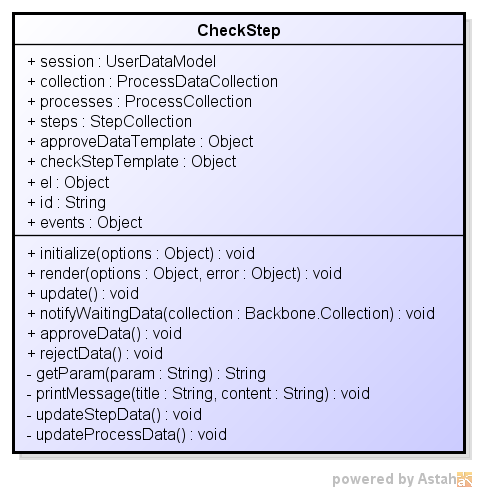
\includegraphics[width=%
\textwidth]
{./classi/client/presenter/po/CheckStep.png} \caption{Diagramma classe  \textit{CheckStep}}
\end{figure}

\begin{flushleft}
\begin{itemize}
\item \textbf{Descrizione:} Classe che ha il compito di definire la logica del controllo di un passo che richiede intervento umano per essere approvato;
\item \textbf{Relazioni con altri componenti:}
\begin{sloppypar}
La classe comunica con il \textit{template} \texttt{\viewAdmin{}.I\fshyp{}Check\fshyp{}Step} per la realizzazione dell'interfaccia grafica, e con le classi \texttt{\collection{}.Pro\fshyp{}cess\fshyp{}Da\fshyp{}ta\fshyp{}Col\fshyp{}lec\fshyp{}tion} e \texttt{\model{}.Pro\fshyp{}cess\fshyp{}Mo\fshyp{}del} per gestire e ottenere i dati dal \textit{server\ped{G}}.
\end{sloppypar}
\item \textbf{Attributi:}
\begin{sloppypar}
\begin{itemize}
\item \texttt{+ ProcessDataCollection processdata:}\\ campo dati di tipo \texttt{\collection{}.Pro\fshyp{}cess\fshyp{}Da\fshyp{}ta\fshyp{}Col\fshyp{}lec\fshyp{}tion} che contiene i dati inviati dagli utenti in attesa di approvazione;
\item \texttt{+ Object template:}\\ oggetto ridefinito da \texttt{Backbone.View}, che contiene il \textit{template HTML\ped{G}} associato alla classe;
\item \texttt{+ Object el:}\\ oggetto ridefinito da \texttt{Backbone.View} che rappresenta l'elemento \textit{HTML\ped{G}} entro cui la classe ascolta eventi generati dagli utenti;
\item \texttt{+ String id:}\\ campo dati ridefinito da \texttt{Backbone.View} contente l'id della classe;
\end{itemize}
\end{sloppypar}
\item \textbf{Metodi:}
\begin{sloppypar}
\begin{itemize}
\item \texttt{+ void initialize():}\\ metodo ridefinito da \texttt{Backbone.View}, invocato alla costruzione di ciascun oggetto della classe, che consente di aggiungere una pagina \textit{HTML\ped{G}} associata al componente;
\item \texttt{+ void render():}\\ metodo ridefinito da \texttt{Backbone.View}, che consente di aggiungere alla pagina \textit{HTML\ped{G}} il \textit{template} campo dati della classe;
\item \texttt{+ void update():}\\ aggiorna il campo dati \texttt{processData} comunicando con il \textit{server\ped{G}};
\item \texttt{+ String getParam(String param):}\\ ritorna il valore del parametro \textit{param} se presente nella \textit{URL\ped{G}};
\item \texttt{+ void approveData():}\\ salva nel \textit{server} lo stato "approvato" ai dati della collezione \textit{processData} dei quali il \textit{process owner\ped{G}} ha richiesto l'approvazione;
\item \texttt{+ void rejectData():}\\ salva nel \textit{server} lo stato "approvato" ai dati della collezione \textit{processData} che il \textit{process owner\ped{G}} ha respinto;
\end{itemize}
\end{sloppypar}
\end{itemize}
\end{flushleft}